	%Analyse_Samlet
\section{Analyse}
Øvelsen er opdelt i to dele, 1. og 2. ordens lavpasfilter.

%Analyse af 1. ordens lavpasfilter
\subsection{Analyse af 1. ordens lavpasfilter}
Figur \ref{lavpasfilter} viser et 1. ordens lavpasfilter med en modstand og en kondensator. $V_{in}$ er stepinput med spænding 0 – 5 V. Steppet sker til tiden t=0 sek.


\begin{equation}
 V_{in}(t) =
  \begin{cases}
    0 & \quad \text{if } t <0\\
    V_{0}&\quad \text{if } t >0\\
  \end{cases}
\label{V_in(t)}\\
\end{equation}
\begin{center}
Ligning: \ref{V_in(t)} Indgangs spændingen er en funktion af t
\end{center}


\begin{figure}[h]
%[h] = sæt billede ind efter midt i tekst
\begin{center}
%rykker billedet ind på midten
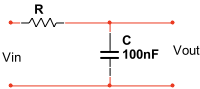
\includegraphics[height=5cm]{M_Fig/Ana_1_Ordens_Lavpasfilter}
\caption{Første ordens lavpasfilter}
%Figur navn
\label{lavpasfilter}
%Bruges ved \ref{•}
\end{center}
\end{figure}





Strøm-spænding sammenhængen for en modstand og en kondensator er:


Modstand:
\begin{equation}
 V_{R} =R\cdot i
\label{Modstand}\\
\end{equation}
\begin{center}
Ligning \ref{Modstand}: Spændingen over en modstand
\end{center}
%\cdot = *
%\frac{1}{2} = 1/2
%V_{Out} = sub

Kondensator:
\begin{equation}
 i =C\cdot \frac{d(V_{C})}{dt}
\label{Kondensator}\\
\end{equation}
\begin{center}
Ligning \ref{Kondensator}: Strømen gennem en kondensator
\end{center}

Output spænding:
\begin{equation}
V_{Out}(t) = V_{C}(t)
\label{V_out=V_C}\\
\end{equation}
\begin{center}
Ligning \ref{V_out=V_C}: Spændingen over $V_ {C}(t)$ er den samme som i punktet $V_{Out}(t)$
\end{center}




Følgende 8 delopgaver er givet:
\subsubsection*{1. Vis ved Kirchhoffs love : KVL}
Vis ved Kirchhoffs love at følgende differentialligning gælder for kredsløbet i Figur \ref{lavpasfilter} : 
\begin{equation}
V_{in}(t)= R \cdot C \cdot \frac{d(V_{out}(t))}{dt} + V_{out}(t)
\label{dfLigning}\\
\end{equation}

Efter en kredsløbsanalyse ses det at:
\begin{center}
\begin{equation}
V_{in}=V_{R}+V_{C}
\label{V_in:KVL}
\end{equation}
\end{center}
 
 Ved brug af Ligning \ref{V_in(t)} og Ligning \ref{V_out=V_C}  kan ligningen omskrives til 
 \begin{center}
\begin{equation}
V_{0}=V_{R}+V_{Out}
\label{V_0:KVL}
\end{equation}
\end{center}

Ved at kombinere Ligning \ref{Modstand} og Ligning \ref{Kondensator}, kan der findes et nyt udtryk fra $V_{R}$ som er afhængig af tiden t
\begin{equation}
	V_{R} = R\cdot C\cdot \dfrac{d}{dt}\cdot V_{C}
\end{equation}

Dernæst kan den indsættes i Ligning \ref{V_0:KVL} hvilket medføre 
\begin{equation}
 V_{0}= R \cdot C \cdot \frac{d(V_{out}(t))}{dt} + V_{out}(t)
\end{equation}
	
\subsubsection*{2. Løs differentialligningen med hensyn til Vout }
 Løs differentialligningen med hensyn til Vout for $ 0\leq t<\infty$
 
 Ligning \ref{dfLigning} kan omskrives så konstanten foran $\frac{d(V_{out}(t))}{dt}$ ved at gange igennem med $\frac{1}{R \cdot C}$, det medføre 
\begin{equation}
\frac{d(V_{out}(t))}{dt}+\frac{1}{R \cdot C}\cdot V_{out}(t) =\frac{1}{R \cdot C} \cdot V_{0}
\label{DL1_alm.}
\end{equation} 

Ved hjælp af en løsnings protokol Ligning \ref{DL1_alm.} nu løses:

\begin{equation}
P(t) = \frac{1}{R \cdot C}
\end{equation}

\begin{equation}
Q(t) = \frac{1}{R \cdot C}\cdot V_{0}
\end{equation}

\begin{center}
\begin{equation}
\mu(t) = e^{\int{P(t) dt}}\rightarrow e^{(\frac{t}{R \cdot C})}
\label{Helpfunktion}
\end{equation}
Ligning \ref{Helpfunktion}: Hjælpefunktion
\end{center}

\begin{center}
\begin{equation}
F(t)=\int{\mu(t) \cdot Q(t) dt}\rightarrow V_{0}+k \cdot e^{-\frac{t}{R \cdot C}}
\label{Stamfunktion}
\end{equation}
Ligning \ref{Stamfunktion}: Stamfunktion
\end{center}

\begin{center}
\begin{equation}
V_{Out}(t) = \frac{1}{\mu(t)} \cdot (F(t)+k) \xrightarrow[ ]{simplify} V_{0}+k \cdot e^{-\frac{t}{R \cdot C}}
\label{Fuldstendig losning}
\end{equation}
Ligning \ref{Fuldstendig losning}: Fuldstændig løsning
\end{center}

\begin{center}
\begin{equation}
k=V_{Out}(0) \xrightarrow[ ]{solve,k}-V_{0}
\label{Betingelse} 
\end{equation}
Ligning \ref{Betingelse}: Betingelse
\end{center}

\begin{center}
\begin{equation}
V_{Out}(t)=V_{0}-V_{0} \cdot e^{\frac{-t}{R \cdot C}}
\label{Specifikke losning}
\end{equation}
Ligning \ref{Specifikke losning}: Specifikke Løsning
\end{center}

 
\subsubsection*{3. Beregn tidskonstanten}
Beregn tidkonstanten %τ
 for lavpasfilteret med hhv.%R= 10 kΩ og R=100 kΩ.
 
 Her skal jeg skrive videre i morgen

\subsubsection*{4. Beregn kurveform}
Beregn kurveform for Vout med hhv. $R= 10 k\Omega$ og  $R=100 k\Omega$, 
og vis disse grafisk for %0 ≤t≤50 ms 

\subsubsection*{5. Beregn Vout max}
Beregn den maksimale værdi af Vout i de to tilfælde.

\subsubsection*{6. Bestem stigetiden tr}
Bestem stigetiden tr %(10-90%).

\subsubsection*{7. Forklar}
Forklar hvordan tidskonstanten og stigetiden kan findes ud fra grafen for 	Vout, og opstil en ligning til bestemmelse af C, når tidskonstanten %τ
 og modstanden R er kendte.

\subsubsection*{8. Indfør resultatur i Tabel 1}
Resultaterne indføres i Tabel 1.





\begin{comment}

	1. Vis ved Kirchhoffs love at følgende differentialligning gælder for kredsløbet i Figur 1 :
 
	

	2. Løs differentialligningen med hensyn til Vout for 0 ≤t<∞

	3. Beregn tidkonstanten τ for lavpasfilteret med hhv. R= 10 kΩ og R=100 kΩ.

	4. Beregn kurveform for Vout med hhv. R= 10 kΩ og R=100 kΩ, og vis disse grafisk for 0 ≤t≤50 ms 

	5. Beregn den maksimale værdi af Vout i de to tilfælde.

	6. Bestem stigetiden tr (10-90%).

	7. Forklar hvordan tidskonstanten og stigetiden kan findes ud fra grafen for 	Vout, og opstil en ligning til bestemmelse af C, når tidskonstanten τ og modstanden R er kendte.

	8. Resultaterne indføres i Tabel 1.

\end{comment}




% Please add the following required packages to your document preamble:
% \usepackage{booktabs}
\newgeometry{top=1 in, bottom=1 in, left=0.2 in, right= 0.2 in}

\begin{center}
\begin{table}[]
\caption{Multirow table.}
    \label{tab:table1}
    
\begin{tabular}{|c|c|c|c|c|c|c|c|c|c|c|c|}
\hline

\rowcolor[gray]{.6}
 
 \multicolumn{4}{|c|}{\textbf{Analyse}}&\multicolumn{4}{c|}{\textbf{Simulering}}&\multicolumn{4}{c|}{\textbf{Måling}}\\ \hline
 
      \multicolumn{1}{|c|}{\multirow{1}{*}{R }} & \multicolumn{1}{c|}{\multirow{1}{*}{$\tau$ }}  & \multicolumn{1}{c|}{\multirow{1}{*}{$t_{r}$ }}   & \multicolumn{1}{c|}{\multirow{1}{*}{$V_{Max}$ }}  &  \multicolumn{1}{c|}{\multirow{1}{*}{R }} & \multicolumn{1}{c|}{\multirow{1}{*}{$\tau$ }}  & \multicolumn{1}{c|}{\multirow{1}{*}{$t_{r}$ }}   & \multicolumn{1}{c|}{\multirow{1}{*}{$V_{Max}$ }}  &  \multicolumn{1}{c|}{\multirow{1}{*}{R }} & \multicolumn{1}{c|}{\multirow{1}{*}{$\tau$ }}  & \multicolumn{1}{c|}{\multirow{1}{*}{$t_{r}$ }}   & \multicolumn{1}{c|}{\multirow{1}{*}{$V_{Max}$ }}  \\ 
      
k$\Omega$  & [msek]  &  [msek] & [V]  & 0[k$\Omega$]  & [msek]   &  [msek] & [V]  & [k$\Omega$]   &  [msek]  &  [msek]  & [V]\\ \hline
\rowcolor[gray]{.8}
    \multicolumn{12}{|c|}{\textbf{ 1. ordens lavpas filter}} \\ \hline 
 
   10  & 1.0 (\ref{dfLigning})   & 2.197   & 4.966 	  &  10 &  1   & 2.08  & 4.97   &  10  &  1.01   &  2.18   & 5.06 \\ \hline 

   100&  10   & 21.972  & 4.966  &  100 & 10.04  &  19.72   & 4.96  &  100 &  9.87  &  21.053  &  4.65  \\\hline 
\rowcolor[gray]{.8}
    \multicolumn{12}{|c|}{\textbf{ 2. ordens lavpas filter}} \\ \hline 
 
 
   1  & \cellcolor[gray]{.8}   & x1   & x2 	  &  1 &  \cellcolor[gray]{.8}   & x3  & x4   &  1  &  \cellcolor[gray]{.8}   &  x5   & x6 \\ \hline 

   10&  \cellcolor[gray]{.8}   & x7  & x8  &  10 & \cellcolor[gray]{.8}  &  x9   & x10  &  10 &  \cellcolor[gray]{.8}  &  x11  &  x12  \\ \hline 
\end{tabular}
\end{table}
\end{center}


